\documentclass{article}

\usepackage{amsmath, amsthm, amssymb, amsfonts}
\usepackage{thmtools}
\usepackage{graphicx}
\usepackage{setspace}
\usepackage{geometry}
\usepackage{float}
\usepackage{hyperref}
\usepackage[utf8]{inputenc}
\usepackage[english]{babel}
\usepackage{framed}
\usepackage[dvipsnames]{xcolor}
\usepackage{tcolorbox}

\colorlet{LightGray}{White!90!Periwinkle}
\colorlet{LightOrange}{Orange!15}
\colorlet{LightGreen}{Green!15}

\newcommand{\HRule}[1]{\rule{\linewidth}{#1}}

\declaretheoremstyle[name=Theorem,]{thmsty}
\declaretheorem[style=thmsty,numberwithin=section]{theorem}
\tcolorboxenvironment{theorem}{colback=LightGray}

\declaretheoremstyle[name=Proposition,]{prosty}
\declaretheorem[style=prosty,numberlike=theorem]{proposition}
\tcolorboxenvironment{proposition}{colback=LightOrange}

\declaretheoremstyle[name=Principle,]{prcpsty}
\declaretheorem[style=prcpsty,numberlike=theorem]{principle}
\tcolorboxenvironment{principle}{colback=LightGreen}

\setstretch{1.2}
\geometry{
    textheight=9in,
    textwidth=5.5in,
    top=1in,
    headheight=12pt,
    headsep=25pt,
    footskip=30pt
}

% ------------------------------------------------------------------------------

\begin{document}

% ------------------------------------------------------------------------------
% Cover Page and ToC
% ------------------------------------------------------------------------------

\title{ \normalsize \textsc{}
\\ [2.0cm]
\HRule{1.5pt} \\
\LARGE \textbf{\uppercase{Documento de Casos de Uso}
\HRule{2.0pt} \\ [0.6cm] \LARGE{Inventario del Cuarto} \vspace*{10\baselineskip}}
}
\date{}
\author{\textbf{Ricardo Emmanuel Uriegas Ibarra}}

\maketitle
% remove page number from the cover page
\thispagestyle{empty} % Quita el número de página en esta página
\newpage

\tableofcontents
\newpage

% ------------------------------------------------------------------------------

\section{Introduction}
\subsection{Propósito del Documento}
El objetivo de este documento es describir los requisitos funcionales y no funcionales del \textit{Sistema de Inventario del Cuarto}. Los requisitos aquí documentados son el resultado de entrevistas y validaciones con el cliente; con el propósito de asegurar cubre las necesidades correspondientes.

\subsection{Alcance del Sistema}
El sistema permitira gestionar de mejor manera el inventario de items del dormitorio. La solucion proposiona una interfaz moderna y amigable para el usuario.

\newpage
\section{Requisitos Funcionales}

\subsection{RF1. Gestionar Items}
\begin{itemize}
    \item Descripción: El sistema permitirá al usuario agregar, modificar y eliminar items del inventario.
    \item Regla: El usuario debe estar autenticado para realizar esta acción.
\end{itemize}

\subsection{RF2. Gestionar Muebles}
\begin{itemize}
    \item Descripción: El sistema permitirá al usuario agregar, modificar y eliminar muebles.
    \item Regla: El usuario debe estar autenticado para realizar esta acción.
\end{itemize}

\subsection{RF3. Gestionar Inmuebles}
\begin{itemize}
    \item Descripción: El sistema permitirá al usuario agregar, modificar y eliminar inmuebles.
    \item Regla: El usuario debe estar autenticado para realizar esta acción.
\end{itemize}

\subsection{RF4. Gestionar Categorías}
\begin{itemize}
    \item Descripción: El sistema permitirá al usuario agregar, modificar y eliminar categorías.
    \item Regla: El usuario debe estar autenticado para realizar esta acción.
\end{itemize}

\subsection{RF5. Gestionar Ubicaciones}
\begin{itemize}
    \item Descripción: El sistema permitirá al usuario agregar, modificar y eliminar ubicaciones.
    \item Regla: El usuario debe estar autenticado para realizar esta acción.
\end{itemize}

\subsection{RF6. Buscar Item}
\begin{itemize}
    \item Descripción: El sistema permitirá al usuario buscar items en el inventario.
    \item Regla: El usuario debe estar autenticado para realizar esta acción.
\end{itemize}

\newpage
\section{Requisitos No Funcionales}

\subsection{RFN1. Usabilidad}
\begin{itemize}
    \item Descripción: La interfaz de usuario debe ser amigable y fácil de usar.
    \item Regla: La interfaz debe ser intuitiva y fácil de usar.
\end{itemize}

\subsection{RFN2. Seguridad}
\begin{itemize}
    \item Descripción: El sistema debe ser seguro.
    \item Regla: La información del usuario debe ser encriptada.
\end{itemize}

\subsection{RFN3. Rendimiento}
\begin{itemize}
    \item Descripción: El sistema debe ser rápido.
    \item Regla: El sistema debe responder en menos de 5 segundos debido a que se mantiene de manera local.
\end{itemize}

\subsection{RFN4. Mantenibilidad}
\begin{itemize}
    \item Descripción: El sistema debe ser fácil de mantener y actualizar.
    \item Regla: El código debe estar bien documentado y seguir estándares de codificación.
\end{itemize}

\subsection{RFN5. Compatibilidad}
\begin{itemize}
    \item Descripción: El sistema debe ser compatible con diferentes dispositivos y navegadores.
    \item Regla: El sistema debe funcionar correctamente en dispositivos móviles y de escritorio, así como en los navegadores más comunes.
\end{itemize}

\newpage

\section{Casos de Uso}

\subsection{CU1. Gestionar Items}
\begin{table}[H]
    \centering
    \begin{tabular}{|l|p{10cm}|}
        \hline
        \textbf{Descripción} & El usuario podrá agregar, modificar y eliminar items del inventario. \\ \hline
        \textbf{Actores} & Usuario \\ \hline
        \textbf{Precondición} & El usuario debe estar autenticado. \\ \hline
        \textbf{Postcondición} & El item se agrega, modifica o elimina del inventario. \\ \hline
        \textbf{Flujo Principal} & 
        \begin{enumerate}
            \item El usuario selecciona la opción de gestionar items.
            \item El sistema muestra la lista de items actuales.
            \item El usuario elige agregar, modificar o eliminar un item.
            \item El sistema procesa la acción solicitada y actualiza el inventario.
        \end{enumerate} \\ \hline
        \textbf{Flujos Alternativos} & 
        \begin{enumerate}
            \item Si el usuario no está autenticado, el sistema solicita iniciar sesión.
            \item Si hay errores en la entrada de datos, el sistema muestra mensajes de error.
        \end{enumerate} \\ \hline
        \textbf{Requisitos Relacionados} & RF1 Gestionar Items \\ \hline
    \end{tabular}
    \caption{Caso de Uso CU1: Gestionar Items}
\end{table}

\subsection{CU2. Gestionar Muebles}
\begin{table}[H]
    \centering
    \begin{tabular}{|l|p{10cm}|}
        \hline
        \textbf{Descripción} & El usuario podrá agregar, modificar y eliminar muebles del inventario. \\ \hline
        \textbf{Actores} & Usuario \\ \hline
        \textbf{Precondición} & El usuario debe estar autenticado. \\ \hline
        \textbf{Postcondición} & El mueble se agrega, modifica o elimina del inventario. \\ \hline
        \textbf{Flujo Principal} & 
        \begin{enumerate}
            \item El usuario selecciona la opción de gestionar muebles.
            \item El sistema muestra la lista de muebles actuales.
            \item El usuario elige agregar, modificar o eliminar un mueble.
            \item El sistema procesa la acción solicitada y actualiza el inventario.
        \end{enumerate} \\ \hline
        \textbf{Flujos Alternativos} & 
        \begin{enumerate}
            \item Si el usuario no está autenticado, el sistema solicita iniciar sesión.
            \item Si hay errores en la entrada de datos, el sistema muestra mensajes de error.
        \end{enumerate} \\ \hline
        \textbf{Requisitos Relacionados} & RF2 Gestionar Muebles \\ \hline
    \end{tabular}
    \caption{Caso de Uso CU2: Gestionar Muebles}
\end{table}

\subsection{CU3. Gestionar Inmuebles}
\begin{table}[H]
    \centering
    \begin{tabular}{|l|p{10cm}|}
        \hline
        \textbf{Descripción} & El usuario podrá agregar, modificar y eliminar inmuebles del inventario. \\ \hline
        \textbf{Actores} & Usuario \\ \hline
        \textbf{Precondición} & El usuario debe estar autenticado. \\ \hline
        \textbf{Postcondición} & El inmueble se agrega, modifica o elimina del inventario. \\ \hline
        \textbf{Flujo Principal} & 
        \begin{enumerate}
            \item El usuario selecciona la opción de gestionar inmuebles.
            \item El sistema muestra la lista de inmuebles actuales.
            \item El usuario elige agregar, modificar o eliminar un inmueble.
            \item El sistema procesa la acción solicitada y actualiza el inventario.
        \end{enumerate} \\ \hline
        \textbf{Flujos Alternativos} & 
        \begin{enumerate}
            \item Si el usuario no está autenticado, el sistema solicita iniciar sesión.
            \item Si hay errores en la entrada de datos, el sistema muestra mensajes de error.
        \end{enumerate} \\ \hline
        \textbf{Requisitos Relacionados} & RF3 Gestionar Inmuebles \\ \hline
    \end{tabular}
    \caption{Caso de Uso CU3: Gestionar Inmuebles}
\end{table}

\subsection{CU4. Gestionar Categorías}
\begin{table}[H]
    \centering
    \begin{tabular}{|l|p{10cm}|}
        \hline
        \textbf{Descripción} & El usuario podrá agregar, modificar y eliminar categorías de los ítems. \\ \hline
        \textbf{Actores} & Usuario \\ \hline
        \textbf{Precondición} & El usuario debe estar autenticado. \\ \hline
        \textbf{Postcondición} & La categoría se agrega, modifica o elimina del inventario. \\ \hline
        \textbf{Flujo Principal} & 
        \begin{enumerate}
            \item El usuario selecciona la opción de gestionar categorías.
            \item El sistema muestra la lista de categorías actuales.
            \item El usuario elige agregar, modificar o eliminar una categoría.
            \item El sistema procesa la acción solicitada y actualiza las categorías.
        \end{enumerate} \\ \hline
        \textbf{Flujos Alternativos} & 
        \begin{enumerate}
            \item Si el usuario no está autenticado, el sistema solicita iniciar sesión.
            \item Si hay errores en la entrada de datos, el sistema muestra mensajes de error.
        \end{enumerate} \\ \hline
        \textbf{Requisitos Relacionados} & RF4 Gestionar Categorías \\ \hline
    \end{tabular}
    \caption{Caso de Uso CU4: Gestionar Categorías}
\end{table}

\subsection{CU5. Gestionar Ubicaciones}
\begin{table}[H]
    \centering
    \begin{tabular}{|l|p{10cm}|}
        \hline
        \textbf{Descripción} & El administrador podrá agregar, modificar y eliminar ubicaciones de los ítems en el inventario. \\ \hline
        \textbf{Actores} & Administrador \\ \hline
        \textbf{Precondición} & El administrador debe estar autenticado. \\ \hline
        \textbf{Postcondición} & La ubicación se agrega, modifica o elimina del inventario. \\ \hline
        \textbf{Flujo Principal} & 
        \begin{enumerate}
            \item El administrador selecciona la opción de gestionar ubicaciones.
            \item El sistema muestra la lista de ubicaciones actuales.
            \item El administrador elige agregar, modificar o eliminar una ubicación.
            \item El sistema procesa la acción solicitada y actualiza las ubicaciones.
        \end{enumerate} \\ \hline
        \textbf{Flujos Alternativos} & 
        \begin{enumerate}
            \item Si el administrador no está autenticado, el sistema solicita iniciar sesión.
            \item Si hay errores en la entrada de datos, el sistema muestra mensajes de error.
        \end{enumerate} \\ \hline
        \textbf{Requisitos Relacionados} & RF5 Gestionar Ubicaciones \\ \hline
    \end{tabular}
    \caption{Caso de Uso CU5: Gestionar Ubicaciones}
\end{table}

\subsection{CU6. Buscar Item}
\begin{table}[H]
    \centering
    \begin{tabular}{|l|p{10cm}|}
        \hline
        \textbf{Descripción} & El usuario podrá buscar ítems dentro del inventario utilizando diferentes criterios de búsqueda. \\ \hline
        \textbf{Actores} & Usuario \\ \hline
        \textbf{Precondición} & El usuario debe estar autenticado. \\ \hline
        \textbf{Postcondición} & Se muestra una lista de ítems que coinciden con los criterios de búsqueda especificados. \\ \hline
        \textbf{Flujo Principal} & 
        \begin{enumerate}
            \item El usuario selecciona la opción de buscar ítem.
            \item El sistema presenta un formulario de búsqueda con diferentes criterios.
            \item El usuario ingresa los criterios de búsqueda y envía la solicitud.
            \item El sistema procesa la solicitud y muestra los resultados que coinciden.
        \end{enumerate} \\ \hline
        \textbf{Flujos Alternativos} & 
        \begin{enumerate}
            \item Si el usuario no está autenticado, el sistema solicita iniciar sesión.
            \item Si no se encuentran ítems que coincidan, el sistema muestra un mensaje indicando que no se encontraron resultados.
            \item Si hay errores en la búsqueda, el sistema muestra mensajes de error.
        \end{enumerate} \\ \hline
        \textbf{Requisitos Relacionados} & RF6 Buscar Item \\ \hline
    \end{tabular}
    \caption{Caso de Uso CU6: Buscar Item}
\end{table}

\newpage
\section{Riesgos Identificados}
\begin{itemize}
    \item R1: El sistema pierde información.
        \subitem \textbf{Mitigación:} Realizar respaldos de la información regularmente.
    \item R2: El sistema se ralentiza.
        \subitem \textbf{Mitigación:} Implementar un sistema de caché y optimizar consultas a la base de datos.
    \item R3: El sistema se desconecta.
        \subitem \textbf{Mitigación:} Conectar una batería de respaldo o un sistema de energía ininterrumpida.
    \item R4: Fallas de seguridad.
        \subitem \textbf{Mitigación:} Implementar medidas de seguridad robustas como cifrado de datos y autenticación de usuarios.
    \item R5: Pérdida de compatibilidad con nuevos dispositivos o navegadores.
        \subitem \textbf{Mitigación:} Realizar pruebas de compatibilidad regularmente y actualizar el sistema según sea necesario.
    \item R6: Errores en el software.
        \subitem \textbf{Mitigación:} Realizar pruebas exhaustivas y mantener un proceso de corrección de errores eficiente.
\end{itemize}

\newpage
\section{Aprobación del Documento}
Este documento ha sido revisado y validado
% tabla de aprobación
\begin{table}[H]
    \centering
    \begin{tabular}{|c|c|c|c|}
        \hline
        \textbf{Nombre} & \textbf{Rol} & \textbf{Firma} & \textbf{Fecha} \\
        \hline
        Ricardo Uriegas & Responsable del Proyecto & &  \\
        \hline
    \end{tabular}
\end{table}

\newpage
\section{Conclusión}
El presente documento ha detallado los requisitos funcionales y no funcionales del \textit{Sistema de Inventario del Cuarto}, así como los casos de uso y los riesgos identificados asociados al desarrollo e implementación del sistema. A través de una interfaz moderna y amigable, el sistema permitirá a los usuarios gestionar de manera eficiente los items, muebles, inmuebles, categorías y ubicaciones dentro del inventario del dormitorio, garantizando al mismo tiempo altos estándares de usabilidad, seguridad y rendimiento.

La implementación de este sistema facilitará la administración del inventario, reduciendo errores y mejorando la productividad del usuario. Además, se han contemplado medidas de mitigación para los riesgos identificados, asegurando la continuidad y confiabilidad del sistema.

Se espera que, con la adopción de este sistema, se logre una gestión más organizada y efectiva del inventario, adaptándose a las necesidades cambiantes del usuario y garantizando una experiencia de uso óptima.

\newpage
\section{Anexos}
\subsection{Prototipo de la Interfaz}
\begin{figure}[H]
    \center
    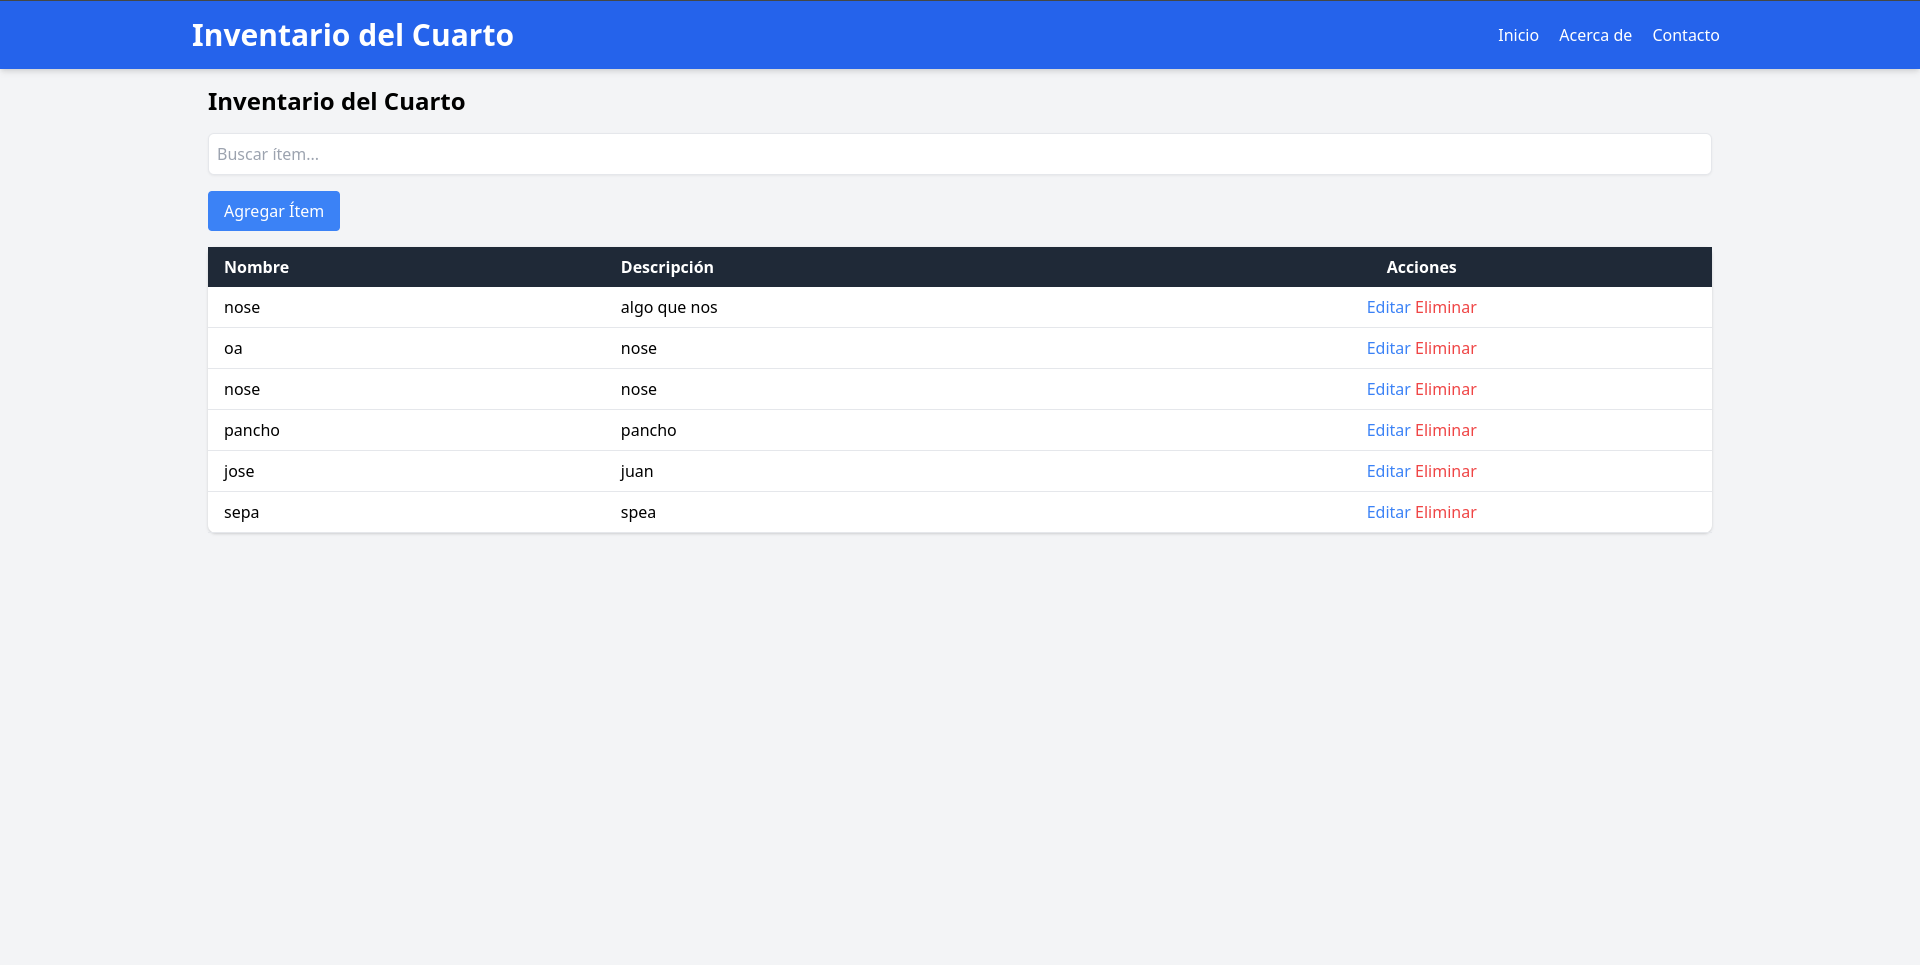
\includegraphics[width=\textwidth]{img/image1.png}
    \caption{Boceto rápido de la interfaz deseada}
\end{figure}

\begin{figure}[H]
    \center
    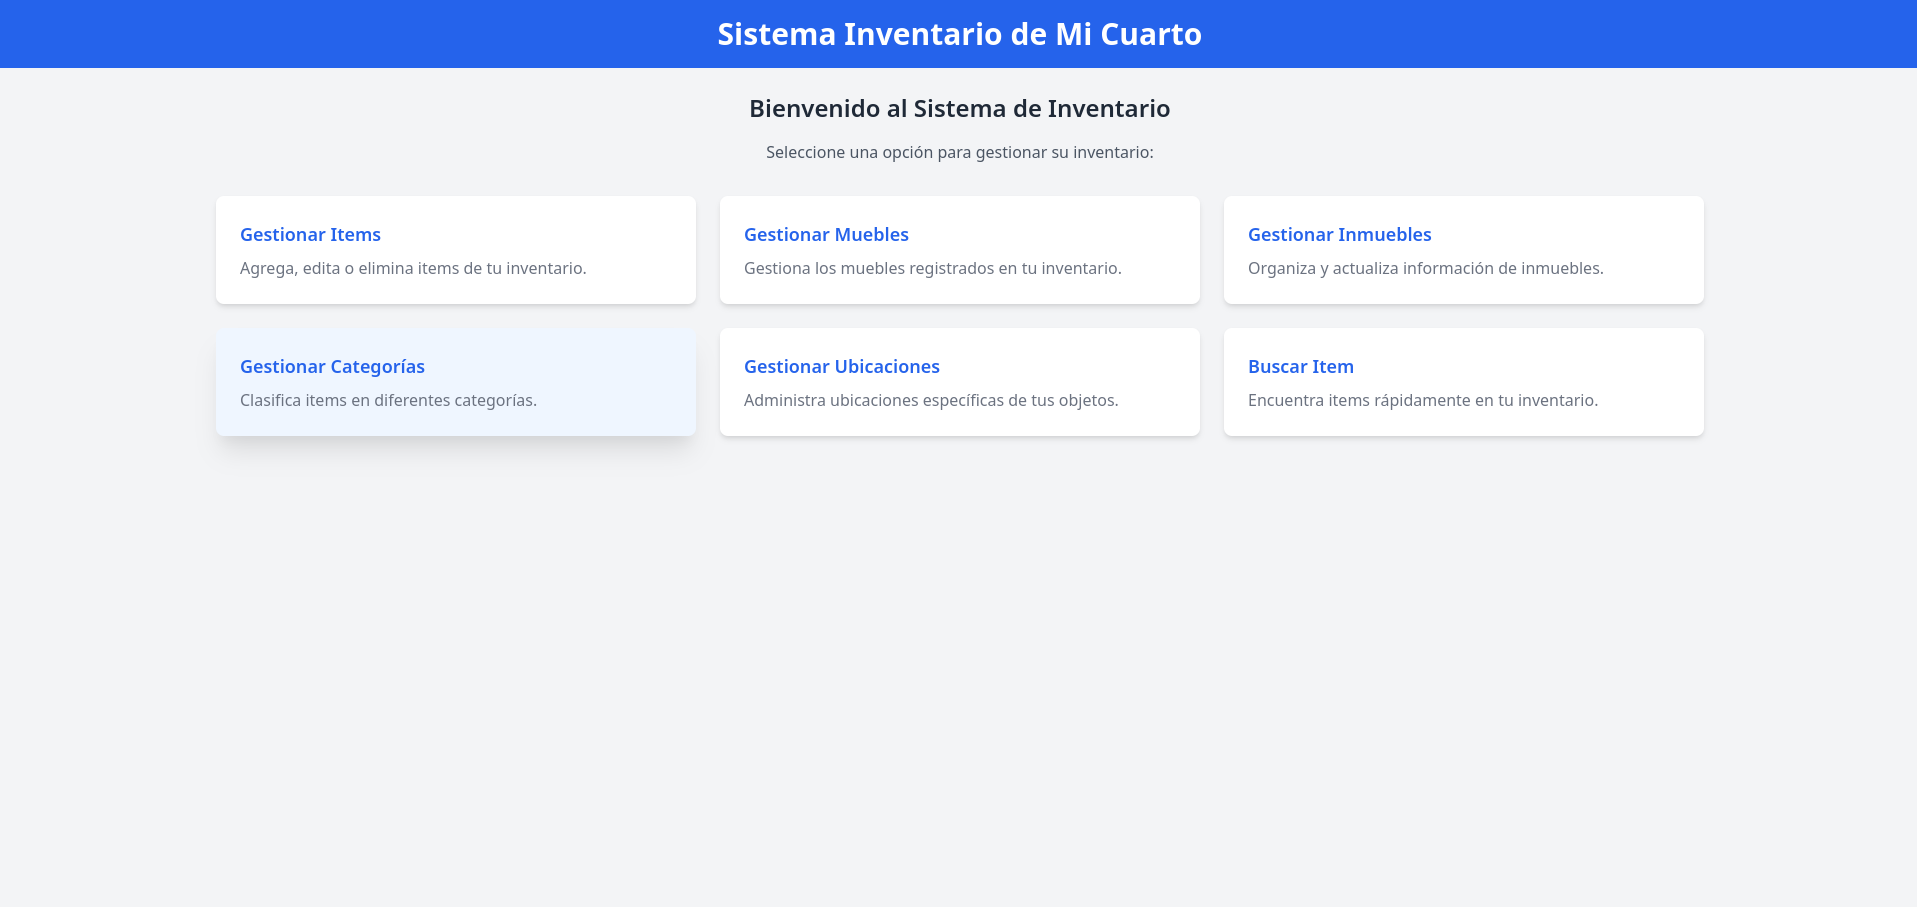
\includegraphics[width=\textwidth]{img/principal.png}
    \caption{Boceto rápido de la interfaz deseada}
\end{figure}

\subsection{Diagrama de Casos de Uso}
\begin{figure}[H]
    \center
    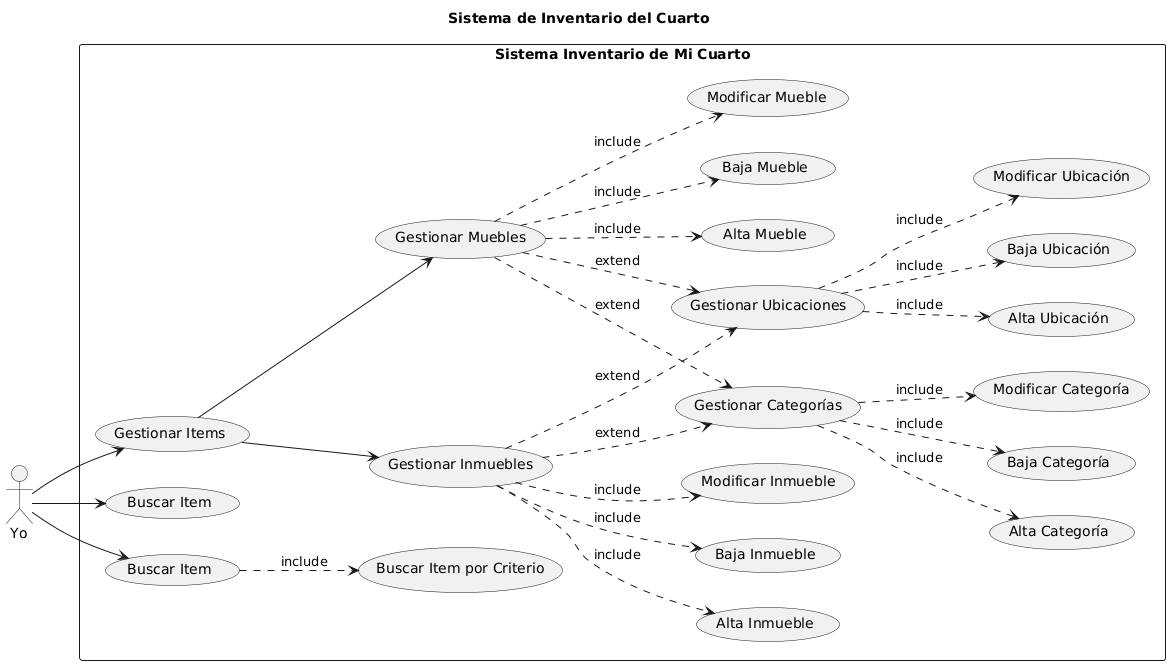
\includegraphics[width=\textwidth]{img/image.png}
    \caption{Diagrama General de Casos de Uso del Proyecto}
\end{figure}

\begin{figure}[H]
    \centering
    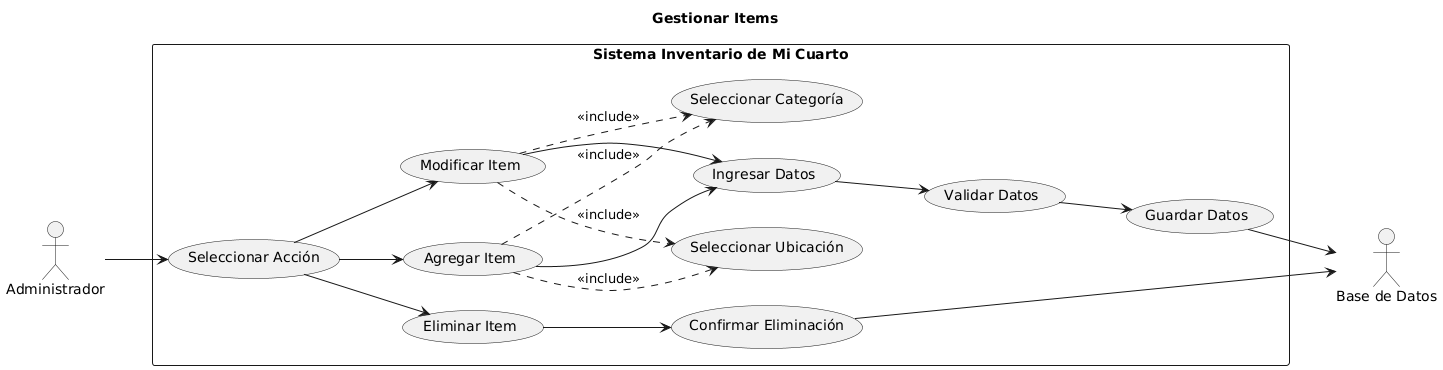
\includegraphics[width=\textwidth]{img/GestionarItems.png}
    \caption{Diagrama de Casos de Uso: Gestionar Items}
\end{figure}

\begin{figure}[H]
    \centering
    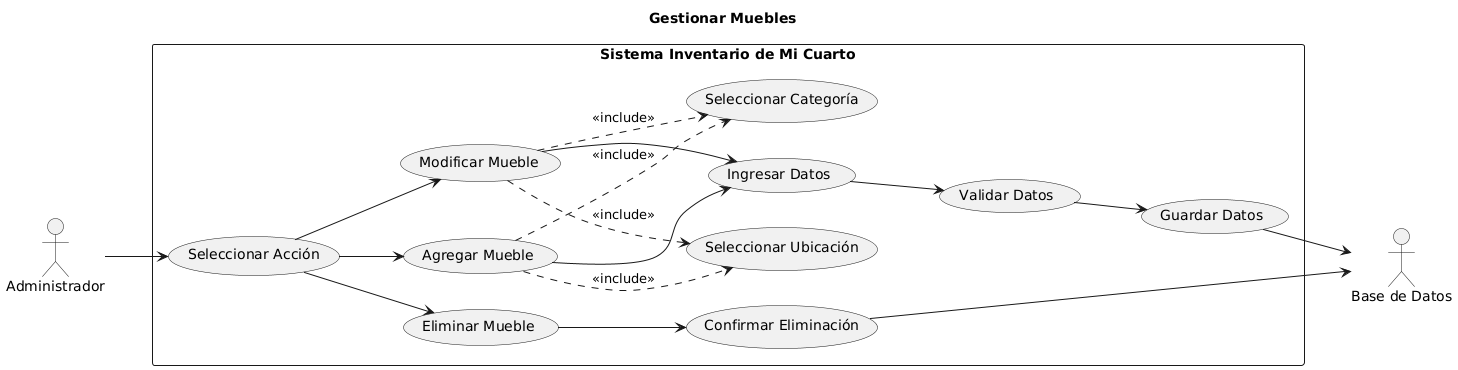
\includegraphics[width=\textwidth]{img/GestionarMuebles.png}
    \caption{Diagrama de Casos de Uso: Gestionar Muebles}
\end{figure}

\begin{figure}[H]
    \centering
    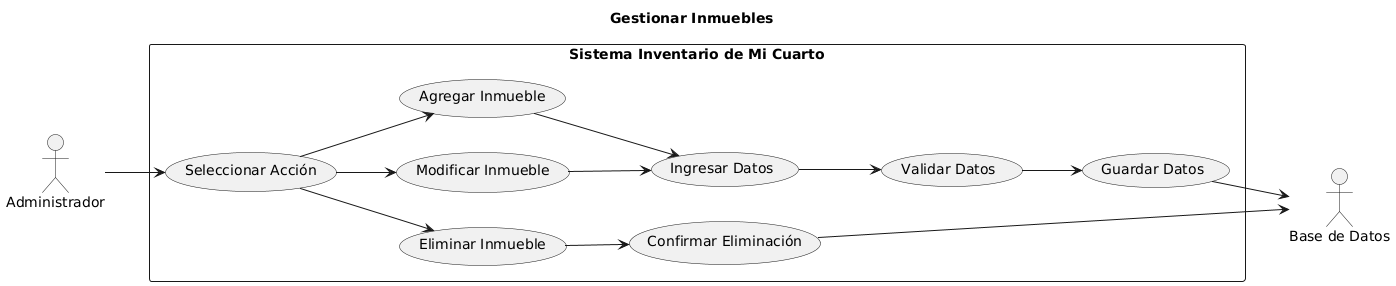
\includegraphics[width=\textwidth]{img/GestionarInmuebles.png}
    \caption{Diagrama de Casos de Uso: Gestionar Inmuebles}
\end{figure}

\begin{figure}[H]
    \centering
    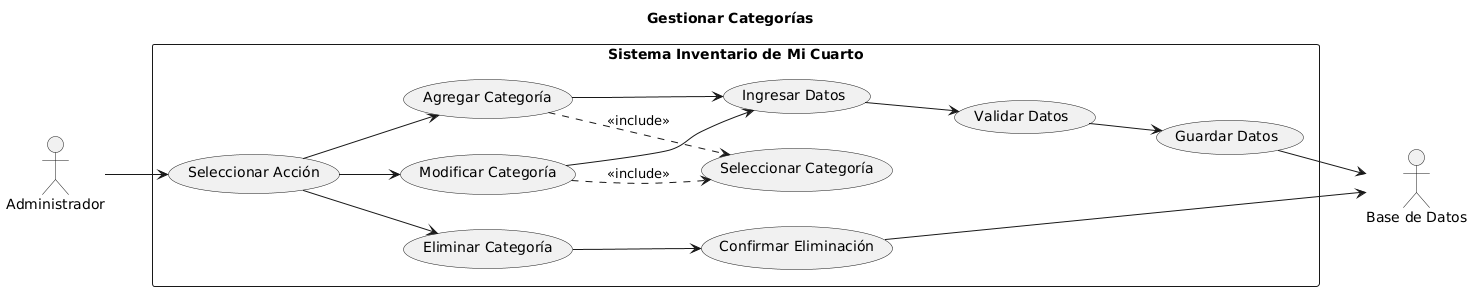
\includegraphics[width=\textwidth]{img/GestionarCategorias.png}
    \caption{Diagrama de Casos de Uso: Gestionar Categorías}
\end{figure}

\begin{figure}[H]
    \centering
    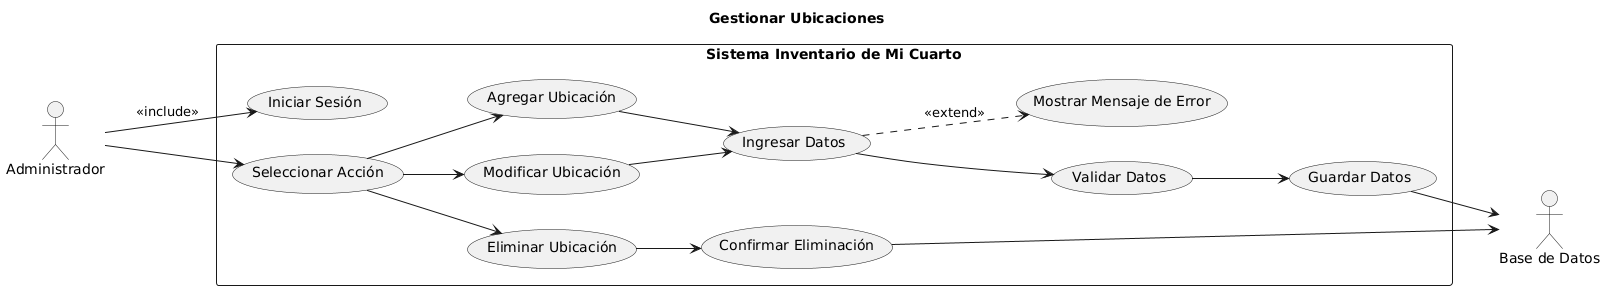
\includegraphics[width=\textwidth]{img/GestionarUbicaciones.png}
    \caption{Diagrama de Casos de Uso: Gestionar Ubicaciones}
\end{figure}

\begin{figure}[H]
    \centering
    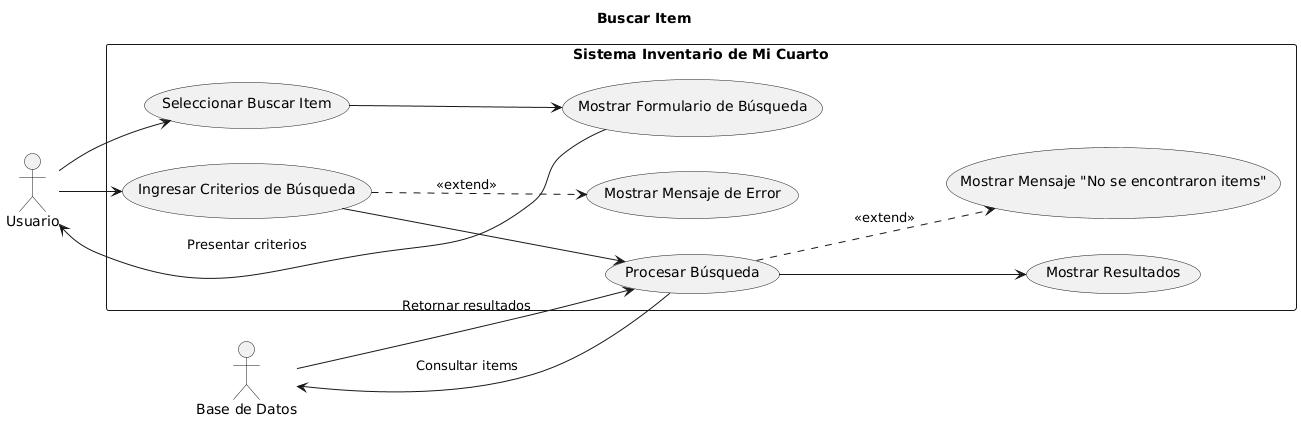
\includegraphics[width=\textwidth]{img/BuscarItem.png}
    \caption{Diagrama de Casos de Uso: Buscar Item}
\end{figure}

% no aplica
\subsection{Diagrama Entidad-Relación}
\begin{figure}[H]
    \center
    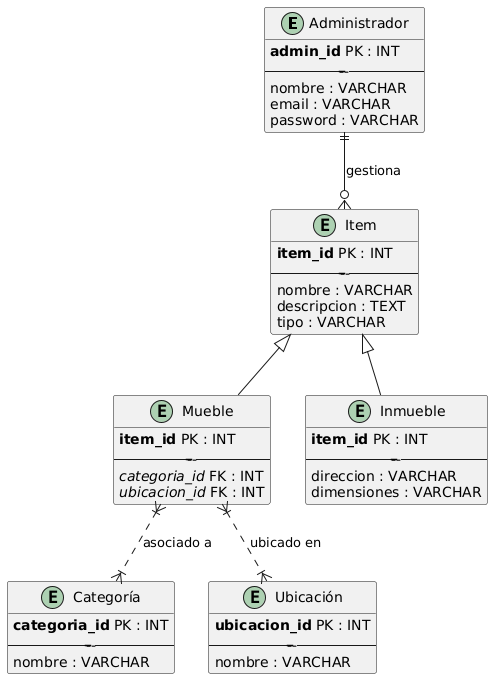
\includegraphics[width=\textwidth]{img/EntidadRelacion.png}
    \caption{Diagrama Entidad-Relación del Sistema}
\end{figure}

\end{document}
